%% 
%% Copyright 2026 Elsevier Ltd
%% 
%% This file is part of the 'Elsarticle Bundle'.
%% ---------------------------------------------
%% 
%% It may be distributed under the conditions of the LaTeX Project Public
%% License, either version 1.2 of this license or (at your option) any
%% later version. The latest version of this license is in
%%  http://www.latex-project.org/lppl.txt
%% and version 1.2 or later is part of all distributions of LaTeX
%% version 1999/12/01 or later.
%% 
%% The list of all files belonging to the 'Elsarticle Bundle' is
%% given in the file `manifest.txt'.
%% 

%% Template article for Elsevier's document class `elsarticle'
%% with numbered style bibliographic references
%% SP 2008/03/01

\documentclass[preprint,12pt, a4paper]{elsarticle}

%% Use the option review to obtain double line spacing
%% \documentclass[authoryear,preprint,review,12pt]{elsarticle}

%% For including figures, graphicx.sty has been loaded in
%% elsarticle.cls. If you prefer to use the old commands
%% please give \usepackage{epsfig}

%% The amssymb package provides various useful mathematical symbols
\usepackage{amssymb}
%% Long code identifiers set in \texttt cannot be hyphenated and overflow the
%% column. These macros give TeX break opportunities at the underscores.
\newcommand{\hte}{\texttt{hines\_\allowbreak tree\_\allowbreak eliminate}}
\newcommand{\ccm}{\texttt{chip\_\allowbreak channel\_\allowbreak multiloop}}
\usepackage{hyperref}
\setlength{\parindent}{0pt}
%% The amsthm package provides extended theorem environments
%% \usepackage{amsthm}

%% The lineno packages adds line numbers. Start line numbering with
%% \begin{linenumbers}, end it with \end{linenumbers}. Or switch it on
%% for the whole article with \linenumbers.
%\usepackage{lineno}

\journal{SoftwareX}
\graphicspath{{figures/}}

\begin{document}
\renewcommand{\labelenumii}{\arabic{enumi}.\arabic{enumii}}

\begin{frontmatter}

%% Title, authors and addresses

%% use the tnoteref command within \title for footnotes;
%% use the tnotetext command for theassociated footnote;
%% use the fnref command within \author or \address for footnotes;
%% use the fntext command for theassociated footnote;
%% use the corref command within \author for corresponding author footnotes;
%% use the cortext command for theassociated footnote;
%% use the ead command for the email address,
%% and the form \ead[url] for the home page:
%% \title{Title\tnoteref{label1}}
%% \tnotetext[label1]{}
%% \author{Name\corref{cor1}\fnref{label2}}
%% \ead{email address}
%% \ead[url]{home page}
%% \fntext[label2]{}
%% \cortext[cor1]{}
%% \address{Address\fnref{label3}}
%% \fntext[label3]{}

\title{GENESIS 2.5: optimisation and opt-in OpenCL/CUDA acceleration for the GENESIS/PGENESIS compartmental neural simulator}

\author[1]{Karol Chlasta\corref{cor1}}
\ead{karol@chlasta.pl}
\author[2]{Grzegorz Marcin W\'ojcik}
\ead{gmwojcik@umcs.edu.pl}

\address[1]{Kozminski University, ul. Jagiello\'nska 57/59, 03-301 Warsaw, Poland; WarsawIQ, Al. Jana Paw\l{}a II 43A/37B, 01-001 Warsaw, Poland}
\address[2]{Maria Curie-Sk{\l}odowska University, ul. Akademicka 9, 20-033 Lublin, Poland}

\cortext[cor1]{Corresponding author.}

\begin{abstract}
GENESIS is a long-established compartmental neural simulator. We release GENESIS~2.5, adding opt-in OpenCL and CUDA backends for the Hodgkin--Huxley channel-update path and \hte{}, a GPU Hines tree-elimination kernel for dendritic trees, leaving every existing model, script and MPI workflow unchanged. On cluster hardware the accelerator reaches $57\times$ end-to-end speedup on a 160\,000-compartment population, matching the fp64 CPU solver to $\sim$$10^{-7}$\,V. Measured against other simulators on one node, it runs the Vogels--Abbott COBAHH benchmark $2.3\times$ faster than CoreNEURON on a single CPU core, and on the GPU it overtakes the GPU-native Arbor beyond 18--64\,ms of simulated time depending on the card; CoreNEURON's GPU stays $1.23\times$ ahead on that spiking benchmark. GENESIS can now run a spiking network on the GPU, though not faster than on the CPU. Its solver handled one spiking cell at a time, so a network needed one solver per cell, 4000 of them for the benchmark used here, and that cost dominated. One solver now holds a whole layer, which by itself makes the CPU arm $1.4\times$ faster. On the GPU the network is no quicker, because the cells exchange spikes every timestep and all 100\,000 steps run as separate GPU calls. The release also makes $O(n^2)$ model construction linear and repairs seven defects, three of them in the solver GENESIS~2.4 ships.
\end{abstract}

\begin{keyword}
GENESIS \sep PGENESIS \sep OpenCL \sep CUDA \sep GPU acceleration \sep compartmental neural simulation \sep Hines solver
\end{keyword}

\end{frontmatter}

%\linenumbers

\section*{Required Metadata}

\section*{Current code version}

\begin{table}[!h]
\begin{tabular}{|l|p{6.0cm}|p{6.0cm}|}
\hline
\textbf{Nr.} & \textbf{Code metadata description} & \textbf{Please fill in this column} \\
\hline
C1 & Current code version & v2.5.1 (2026-08-20; OpenCL + CUDA-validated, multi-compartment GPU Hines solve, spiking networks on the accelerator) \\
\hline
C2 & Permanent GitHub link to code/repository used for this code version & \url{https://github.com/WarsawIQ/genesis-2.5} (archived release: \url{https://doi.org/10.5281/zenodo.22032886}) \\
\hline
C3 & Legal Code License  & GNU General Public License v2 or later (program); GNU Lesser General Public License v2.1 or later (library portions) -- see \texttt{LICENSE} \\
\hline
C4 & Code versioning system used & git \\
\hline
C5 & Software code languages, tools, and services used & C, OpenCL C, CUDA C++ (accelerator backends), MPI (PGENESIS), Python (benchmark analysis/plotting) \\
\hline
C6 & Compilation requirements, operating environments \& dependencies & Linux x86\_64, GCC, GNU make, an OpenCL 1.2+ runtime (tested: ROCm 6.3.1 and Mesa rusticl) or a CUDA 12.x toolkit (tested: CUDA 12.8, \texttt{sm\_80} NVIDIA A100 and \texttt{sm\_86} NVIDIA A40 on the UMCS cluster) for the GPU backends, an MPI implementation for PGENESIS (MPICH/HYDRA or Open~MPI tested on the UMCS cluster) \\
\hline
C7 & If available Link to developer documentation/manual & \texttt{README.md} and \path{paper/docs/REPLICATION.md} in the repository \\
\hline
C8 & Support email for questions & karol@chlasta.pl \\
\hline
\end{tabular}
\caption{Code metadata (mandatory)}
\end{table}

\textbf{Main text}\\
\begin{enumerate}

\item Motivation and significance

Compartmental simulators remain essential where channel kinetics and dendritic geometry cannot be abstracted away. GENESIS~\cite{bower1998} is among the longest-maintained simulators in this class, with PGENESIS extending it to MPI; both are still used in production workflows, scripted in SLI, independent of newer ecosystems.

Modern workstations ship capable integrated GPUs, but GENESIS has no accelerator backend: every channel-kinetics update runs on the CPU whatever hardware is present. A GENESIS or PGENESIS user has no path to accelerator support that does not begin with abandoning their models and scripts.

\textbf{Existing accelerated simulators, and what they ask of a user.} Compartmental simulation on GPUs is not new, and the alternatives are mature. NEURON~\cite{hines1997neuron} is the most widely used simulator in this class; CoreNEURON~\cite{kumbhar2019coreneuron} is its optimised compute engine, which strips the interpreter and runs the same models on GPUs through OpenACC, reaching large speedups on multi-rank and multi-GPU systems. Arbor~\cite{arbor2019} was written from scratch for many-core and GPU hardware, with a performance-portable back end and its own model description. NEST~\cite{gewaltig2007nest} and Brian~2~\cite{stimberg2019brian}, the latter reaching GPUs through GeNN~\cite{yavuz2016genn}, simulate networks of point neurons rather than dendritic morphologies. They are therefore not in the comparison below: NEURON, CoreNEURON and Arbor are the simulators a GENESIS user could move a compartmental model to, and the only ones that would be running the same computation.

Each of these is a strong choice for a new model. None is a path for an existing GENESIS model. CoreNEURON accelerates NEURON's models, not GENESIS's; Arbor and Brian~2 require the model to be re-expressed in their own descriptions; and a GENESIS user's investment is typically in SLI scripts, \texttt{.p} cell files and channel prototypes accumulated over years. Porting is not a mechanical translation --- as this work found, two implementations of the same published benchmark differ enough in channel kinetics and connectivity construction that establishing their equivalence is itself experimental work (Section~3). The gap GENESIS~2.5 addresses is therefore not ``fastest simulator'' but ``acceleration without migration'': the same models and scripts, unchanged, on the hardware the user already has.

\textbf{Contributions.} This work contributes:

\begin{enumerate}
\item Opt-in OpenCL and CUDA backends for the \texttt{hsolve} channel-update path, behind one entry point, leaving every existing CPU, MPI, model and SLI-script workflow unchanged.
\item \hte{}, a GPU tridiagonal (Hines~\cite{hines1984efficient}) elimination kernel extending acceleration from isopotential cells to axially-coupled dendritic trees, running the identical elimination the CPU solver does.
\item Seven correctness fixes to released code, none of which requires a user to change a model. Three are in the Hines solver GENESIS~2.4 distributes and reach every multi-neuron \texttt{hsolve}, accelerator or not: \texttt{inject}-driven voltage transients were silently suppressed for all but the first neuron. Four are in the accelerator as first released, where a model using synaptic channels, a \texttt{spike} element, GHK or concentration pools could be dispatched to the GPU and returned wrong voltages with no error raised; such models are now detected at \texttt{SETUP} and computed on the CPU.
\item A latent $O(n^2)$ model-construction bottleneck, unrelated to accelerator support, reduced to linear.
\item A head-to-head evaluation against NEURON, CoreNEURON and Arbor, on a published network model and on a multi-compartment population, with the competing simulators' GPU backends included and the equivalence of the independent implementations verified rather than assumed.
\end{enumerate}

Why a GPU helps here is specific to the workload. In a Hodgkin--Huxley model the per-compartment gating integration dominates the cost and is embarrassingly parallel: each compartment advances from its own voltage and its own table lookups, uncoupled from every other within the step. The state is small and the arithmetic intensity low, so the work maps onto thousands of lightweight threads. That makes the channel-update path the natural first target, ahead of the tridiagonal solve.

We provide both backends because they buy different things. OpenCL is vendor-neutral and runs on the integrated GPUs shipped with ordinary workstations, including devices without double precision, which is why the kernel is fp32 throughout. CUDA targets the datacenter cards where most cluster time is available and the profiling tools are standard. Both sit behind one entry point, so the choice is a build flag and neither the model nor its SLI script changes.

We name this release ``2.5'' rather than ``3.0'' deliberately: ``GENESIS 3''~\cite{g3_dev_plans} produced independent successor lines (Neurospaces/Heccer~\cite{cornelis2011}, MOOSE) evolving into the CBI federation~\cite{cornelis2008cbi,cornelis2007dendrite,cornelis2013interop}, not a single artifact comparable to GENESIS 2.4. This release is not a re-architecture.

\item Software description

\begin{enumerate}
  \item Software architecture

  GENESIS 2.5 leaves the existing architecture (SLI interpreter, \texttt{hsolve} solver, PGENESIS MPI partitioning) unmodified and adds one component: an OpenCL backend invoked from \texttt{hsolve} when an attached element uses \texttt{chanmode=4} (or 5) with real ion-channel state. Two dispatch modes are implemented:
  \begin{itemize}
    \item \emph{Per-step dispatch} (\texttt{ocl\_chip\_update}): one {\small\texttt{clEnqueue\allowbreak NDRange\allowbreak Kernel}} call per simulation step, with channel state uploaded and downloaded every step.
    \item \emph{Multiloop dispatch} (\ccm{}, via \path{GENESIS_OCL_MULTILOOP=<K>}): a single kernel dispatch runs all $K$ steps in an inner GPU-side loop, amortising the per-step PCIe transfer cost that otherwise dominates wall time (Section~3).
  \end{itemize}
  Every accelerator run emits a non-empty profiling summary, which guards against two silent failures: an \texttt{hsolve} with no attached channels never reaching the kernel, and a kernel that fails to build falling back to CPU unnoticed. The kernel is fp32 throughout, so it runs on runtimes without double-precision support; the rest of \texttt{hsolve} stays \texttt{double}, converting only at the buffer boundary.

  Both dispatch modes update each compartment independently, exact only for single-compartment (isopotential) neurons: a real dendritic tree's compartments are coupled through axial resistance, solved on the CPU by \texttt{hsolve} as a compiled bytecode program performing a bottom-up/top-down Gaussian elimination over the tree's tridiagonal system once per step. We add a third kernel, \hte{} (\path{ocl_channel.cl}; CUDA port in \path{cuda/cuda_channel.cuh}), executing this identical bytecode on the GPU, one thread per disconnected tree (neuron), operating on the same flat opcode/coefficient arrays the CPU solver already builds at \texttt{SETUP} time. Because independent trees never reference each other's rows (the combined program is block-diagonal), threads need no synchronisation. The channel and elimination kernels dispatch back to back on the same queue/stream, so the $K$-step batch still uploads and downloads state once. \path{ocl_hsolve.c}/\path{cuda_hsolve.c} select this path whenever the \texttt{hsolve} contains a multi-compartment tree, leaving the original kernel for single-compartment networks.

  Synaptically coupled spiking networks reach the kernels in this release. \texttt{hsolve} tracked one spike generator per solver, so such a network had to be built as one solver per cell; it now tracks one per compartment, and a whole layer becomes a single solver whose single-compartment solve the channel kernel completes on the device. One boundary remains, and it is a scheduling one rather than a kernel one: a network with zero axonal delay exchanges spikes every step, so multiloop batching does not apply and each step pays a dispatch. Section~3 measures what that costs.

  \item Software functionalities

  \begin{itemize}
    \item Unmodified serial (\texttt{genesis}), headless (\texttt{nxgenesis}), and MPI (PGENESIS) execution paths.
    \item OpenCL channel-update kernel for Hodgkin--Huxley-style \texttt{tabchannel} gating (Na $X^3Y^1$, K $X^4$), dispatched per-step or batched via multiloop.
    \item A CUDA backend at the same call site (\path{genesis/src/hines/cuda/}): a line-for-line fp32 port behind an identical entry point, so one model and harness drive either backend.
    \item Device-side dispatch confirmation distinguishing a genuine GPU run from CPU fallback.
    \item A driven-spiking benchmark (\path{hh_spiking_benchmark.g}) exercising the repaired \texttt{inject} path.
    \item Three corrected Hines-solver defects (forward-elimination fast-path guard, backward-elimination root handling, \path{SET_DIAG}/\path{SKIP_DIAG} row selection), independent of GPU support.
    \item \hte{}, a GPU tridiagonal elimination kernel in both backends, extending acceleration to axially-coupled dendritic trees (Section~3).
    \item Five corrected $O(n^2)$ model-construction defects, restoring linear-time construction independent of GPU support (Section~3).
  \end{itemize}
\end{enumerate}

The tridiagonal kernel decides whether any of this reaches realistic morphologies. Accelerating channel updates alone leaves the axial coupling on the CPU, where the solve becomes the bottleneck as soon as the channel work is taken out of it. Moving it to the device is what lifts acceleration from isopotential point-neuron networks to populations of real dendritic trees, the regime Section~3 measures.

\item Illustrative examples

Every measurement below comes from one of two UMCS ``Lunar'' cluster nodes: inf02, a Xeon Gold 6342 with an NVIDIA A40, and inf03, a Xeon Platinum 8358 with an A100. CPU arms are single-threaded unless stated.

\textbf{Reproducing the GPU multiloop result.} \path{genesis/Scripts/benchmark/hh_spiking_benchmark.g} builds $N$ driven Hodgkin--Huxley neurons under one \texttt{hsolve} (\texttt{chanmode=4}); \path{GENESIS_CUDA_MULTILOOP=}$K$ dispatches all $K$ steps in one GPU call. Both arms are wall-clocked identically at $K=50\,000$ on the A40 and A100.

Table~\ref{tab:cuda} reports both backends after the scheduler and solver fixes; speedup grows with $N$ throughout.





\textbf{Numerical fidelity of the fp32 accelerator.} \path{genesis/Scripts/benchmark/hh1952_ap_verify.g} compares the classic 1952 squid AP across CPU fp64, GPU per-step, and GPU multiloop paths: fp32 agrees with fp64 to $\sim$$2\times10^{-7}$\,V over a single AP, all $N$ neurons identical to $<10^{-6}$\,V (Fig.~\ref{fig:divergence}). Over long spiking runs, fp32/fp64 traces drift in spike \emph{phase} but preserve waveform and firing rate, why timing uses driven neurons while correctness uses a single-AP window.

\begin{figure}[!h]
\centering

\includegraphics[width=0.8\textwidth]{fig_campaign_divergence.png}
\caption{Absolute difference between the accelerator's fp32 membrane voltages and the CPU's fp64 ones, for one driven spiking neuron over 6400 steps. Both dispatch modes are drawn --- one kernel call per step, and one call covering a batch of them --- and they overlap.}
\label{fig:divergence}
\end{figure}

\textbf{CUDA backend on NVIDIA hardware.} The CUDA backend builds from the same source (\texttt{make USE\_CUDA=1}) against the identical harness, and reproduces the fp64 CPU action potential to $7\times10^{-8}$\,V, confirming parity with both the CPU and OpenCL paths. That sweep is 10 replicates on each of the two UMCS cluster GPUs. The two cards are close at every size, and the OpenCL backend trails CUDA by roughly $8\%$ --- about what a faithful port of the same kernels costs, and the price of running on hardware CUDA does not reach.

These are \emph{end-to-end} speedups, and every figure in this paper uses that one definition. Timing the two arms by different clocks inflates the ratio tenfold and can invent differences between cards; measured consistently the A40 and A100 are indistinguishable ($21.0\pm0.3\times$ vs.\ $21.9\pm0.3\times$).

At $N=500$ the accelerator barely pays for itself: fixed costs dominate a run the CPU finishes in under a second.

\begin{table}[!h]
\centering
\small
\begin{tabular}{|r|r|r|r|r|}
\hline
\textbf{$N$} & \multicolumn{2}{c|}{\textbf{NVIDIA A40}} & \multicolumn{2}{c|}{\textbf{NVIDIA A100}} \\
       & \textbf{CUDA} & \textbf{OpenCL} & \textbf{CUDA} & \textbf{OpenCL} \\
\hline
500   & 1.5 $\pm$ 0.1$\times$ & 1.5$\times$ & 1.8 $\pm$ 0.3$\times$ & 1.7$\times$ \\
\hline
5\,000 & 8.7 $\pm$ 0.3$\times$ & 7.5$\times$ & 9.7 $\pm$ 0.4$\times$ & 8.7$\times$ \\
\hline
50\,000 & \textbf{21.0 $\pm$ 0.3}$\times$ & 19.2$\times$ & \textbf{21.9 $\pm$ 0.3}$\times$ & 20.4$\times$ \\
\hline
\end{tabular}
\caption{What each accelerator backend is worth against the CPU solver, and how that changes with population size. Single-compartment multiloop kernel (\texttt{hh\_spiking\_benchmark.g}, $K=50\,000$ steps), fp32 GPU against fp64 CPU on the UMCS cluster. Both arms of every ratio are wall-clocked around the whole process, so construction, transfers and per-step host work sit inside each figure. CUDA is the mean of 10 replicates with propagated uncertainties, OpenCL of 3. Raw data: \protect\path{cluster_bringup/logs/}.}
\label{tab:cuda}
\end{table}

\textbf{Multi-compartment GPU acceleration.} The multiloop kernel above is exact only for single-compartment (isopotential) neurons: for a real dendritic tree it silently drops all axial coupling. \hte{} (Section~2.1) performs this elimination on-device, dispatched whenever the \texttt{hsolve} contains a multi-compartment tree.

\emph{Correctness.} Linear-chain and branching benchmarks compare GPU against fp64 CPU across \texttt{NCOMP}\,$=1$--$32$ and up to $N=10\,000$ neurons: agreement is $\sim$$10^{-7}$\,V, matching single-compartment fidelity. One topology is not handled: a single-compartment branch off a branch point, which violates the kernel bootstrap's seed-row assumption. Both backends detect it at initialisation and compute that \texttt{hsolve} on the CPU, so it costs speed rather than accuracy. A separate platform limit: on an integrated GPU that also drives the display, the tree dispatch trips the driver's reset above $\sim$22\,000 compartments. The same configuration runs on the A40, so \texttt{GENESIS\_OCL\_TREE\_MAX\_NCOMPTS} caps model size there and is 0 on dedicated hardware.

\emph{Speed.} Table~\ref{tab:multicomp} and Fig.~\ref{fig:multicomp_speedup} report speedup (mean $\pm$ std, 10 replicates) on the two UMCS cards, sweeping $N=100$--$50\,000$ at \texttt{NCOMP}\,$=16$, a range unreachable before the model-construction fix (Impact): $N=50\,000$ took $23.8\pm0.3$\,s to build there, versus not finishing before. Branching topology gives statistically indistinguishable speedups and is omitted from the figure.

Two figures per card answer different questions. The \emph{step-phase} speedup times the simulation loop alone and measures what the kernel can do: both cards are slower than CPU at $N\leq500$, pull ahead past $N\approx500$--$1000$, and reach $37.3\pm0.1\times$ (A40) and $80.8\pm1.0\times$ (A100) at $N=50\,000$, neither plateaued. The \emph{end-to-end} speedup wall-clocks the whole process, which is what a user waits for: it is far lower, $3.62\pm0.05\times$ (A40) and $3.90\pm0.07\times$ (A100) at $N=50\,000$. The gap is not a kernel deficiency but Amdahl's law applied to a short run --- at $K=200$ steps the unaccelerated construction phase dominates, and the end-to-end figure climbs toward the step-phase ceiling as $K$ grows. Quoting only the step-phase number would overstate what the accelerator delivers in practice.

The cards nearly coincide end-to-end despite the A100 leading by more than $2\times$ on the step phase: the GPU phases take $7.83$\,s (A40) against $8.06$\,s (A100) at $N=50\,000$. Raw data: \protect\path{cluster_bringup/logs/weekend_campaign_*_20260816_clean.csv} and \protect\path{..._multicomp_walltime_createmap_*_clean.csv}.

\emph{Parallelisation granularity.} \hte{} assigns one GPU thread per tree, so speedup comes from spreading many neurons across threads, not from parallelising elimination \emph{within} a tree. For a single detailed morphology alone ($N=1$), only one thread is active: measured directly, the kernel is $\sim$20--21$\times$ \emph{slower} than the CPU at \texttt{NCOMP}\,$=2000$ and $8000$, stable with tree size as expected for a single-thread bottleneck. The kernel therefore accelerates population-scale simulation (Table~\ref{tab:multicomp}), not the single-detailed-cell regime.

\begin{table}[!h]
\centering
\small
\begin{tabular}{|r|r|r|r|r|r|}
\hline
& & \multicolumn{2}{c|}{\textbf{step-phase}} & \multicolumn{2}{c|}{\textbf{end-to-end}} \\
\hline
\textbf{$N$} & \textbf{total comps} & \textbf{A40} & \textbf{A100} & \textbf{A40} & \textbf{A100} \\
\hline
100   & 1\,600  & 0.2 $\pm$ 0.02 & 0.3 $\pm$ 0.02 & 0.43 $\pm$ 0.05 & 0.61 $\pm$ 0.02 \\
\hline
500   & 8\,000  & 1.1 $\pm$ 0.03 & 1.7 $\pm$ 0.11 & 0.77 $\pm$ 0.02 & 1.04 $\pm$ 0.03 \\
\hline
1\,000 & 16\,000 & 2.0 $\pm$ 0.08 & 3.1 $\pm$ 0.07 & 1.10 $\pm$ 0.08 & 1.46 $\pm$ 0.04 \\
\hline
2\,000 & 32\,000 & 4.5 $\pm$ 0.39 & 6.4 $\pm$ 0.18 & 1.37 $\pm$ 0.06 & 1.57 $\pm$ 0.05 \\
\hline
3\,000 & 48\,000 & 6.7 $\pm$ 0.03 & 12.0 $\pm$ 0.37 & 1.87 $\pm$ 0.07 & 1.89 $\pm$ 0.04 \\
\hline
5\,000 & 80\,000 & 6.9 $\pm$ 0.04 & 14.5 $\pm$ 0.47 & 2.60 $\pm$ 0.06 & 2.66 $\pm$ 0.03 \\
\hline
7\,000 & 112\,000 & 9.8 $\pm$ 0.05 & 22.0 $\pm$ 0.43 & 2.92 $\pm$ 0.05 & 3.08 $\pm$ 0.03 \\
\hline
10\,000 & 160\,000 & 13.7 $\pm$ 0.06 & 30.6 $\pm$ 0.68 & 3.01 $\pm$ 0.04 & 3.23 $\pm$ 0.04 \\
\hline
15\,000 & 240\,000 & 20.3 $\pm$ 0.12 & 42.3 $\pm$ 0.77 & 3.27 $\pm$ 0.05 & 3.52 $\pm$ 0.03 \\
\hline
20\,000 & 320\,000 & 25.3 $\pm$ 0.12 & 51.6 $\pm$ 1.16 & 3.39 $\pm$ 0.04 & 3.71 $\pm$ 0.04 \\
\hline
30\,000 & 480\,000 & 31.9 $\pm$ 0.13 & 66.1 $\pm$ 1.12 & 3.53 $\pm$ 0.05 & 3.87 $\pm$ 0.05 \\
\hline
40\,000 & 640\,000 & 35.2 $\pm$ 0.13 & 75.5 $\pm$ 0.96 & 3.56 $\pm$ 0.04 & 3.90 $\pm$ 0.04 \\
\hline
50\,000 & 800\,000 & 37.3 $\pm$ 0.07 & \textbf{80.8 $\pm$ 1.01} & 3.62 $\pm$ 0.05 & \textbf{3.90 $\pm$ 0.07} \\
\hline
\end{tabular}
\caption{What the tree-elimination kernel is worth on dendritic trees, and how much of it survives into the whole run. Linear chains at \texttt{NCOMP}\,$=16$, batched multiloop ($K=200$, $K=100$ for $N\geq5000$), mean $\pm$ std over 10 replicates. \emph{Step-phase} times the simulation loop alone and measures the kernel; \emph{end-to-end} wall-clocks the whole process including model construction, both arms timed identically (\protect\path{cluster_bringup/54_multicomp_walltime.sh}). The end-to-end runs build the population with one \texttt{createmap}, as network models do. ``--'' = not measured. Raw data: \protect\path{cluster_bringup/logs/}.}
\label{tab:multicomp}
\end{table}

\begin{figure}[!h]
\centering

\includegraphics[width=0.98\textwidth]{fig10_multicompartment_speedup.png}
\caption{Speedup of the tree-elimination kernel over the CPU against population size, 16 compartments per neuron, log-log, mean $\pm$ std over 10 replicates. Colour is the card; solid lines time the simulation loop alone, dashed ones the whole run including model construction, at $K=200$ steps.}
\label{fig:multicomp_speedup}
\end{figure}

\textbf{Population-scale model construction was $O(n^2)$; now $O(n)$.} Pushing toward the $\sim$31\,000-neuron Blue Brain Project scale~\cite{markram2015reconstruction} exposed a defect independent of GPU support: 527\,000 compartments did not finish building within 900\,s. Profiling gave a fitted exponent of $2.31$, traced to five pre-existing linear-scan-per-element patterns in element creation, path resolution and \texttt{hsolve} SETUP, none GPU-specific --- each rescanning siblings, paths or compartments where hashing or amortised growth would do. Fixing all five (Fig.~\ref{fig:construction_scaling}) gives an exponent of $0.99$: that population now builds in $14.6\pm0.2$\,s, and 1.7~million compartments in $51.5\pm0.6$\,s. Output is byte-identical on every validation script, confirming a pure performance fix; full diagnosis in \path{genesis/src/hines/GPU_HINES_SOLVE_DESIGN.md}.

\begin{figure}[!h]
\centering

\includegraphics[width=0.8\textwidth]{fig11_construction_scaling.png}
\caption{Model-construction wall time vs.\ $N$, log-log, before (single replicate) and after (mean $\pm$ std, 3 replicates) the five $O(n^2)$ fixes, extended to $N=100\,000$. The ``before'' series stops at $N=8000$: larger $N$ did not finish within the tested budget.}
\label{fig:construction_scaling}
\end{figure}

\textbf{The multi-compartment figures are a floor set by the benchmark, not a ceiling set by the kernel.} The sweeps above use $K=200$ ($K=100$ for $N\geq5000$), which at $dt=50\,\mu$s is 5--10\,ms of simulated activity, short enough that fixed costs dominate both arms. Repeating the measurement at $N=10\,000$ over a range of $K$ (Table~\ref{tab:mcksweep}) separates them: end-to-end speedup rises from $4.3\times$ at $K=200$ to $57.0\pm0.9\times$ at $K=5000$, and step-phase from $13.7\times$ to $116.2\times$. Both grow because the one-time costs they contain are amortised over more steps: model construction for the end-to-end figure, buffer setup and the single batched dispatch for the step-phase figure.

Fitting fixed and marginal costs separates them: construction takes $\approx$1.3\,s on both arms, while one step costs $2.31\times10^{-2}$\,s on the CPU against $1.42\times10^{-4}$\,s on the GPU, a ratio of $163\times$. At $K=5000$ the GPU still reproduces the CPU voltages to $\sim$$10^{-7}$\,V, so this is amortisation, not skipped work. Table~\ref{tab:multicomp} reports the short-$K$ figures because they are what the standing benchmark measures, but a 250\,ms simulation of this population already reaches $57\times$ end-to-end.

\begin{table}[!h]
\centering
\small
\begin{tabular}{|r|r|r|r|}
\hline
\textbf{$K$ steps} & \textbf{CPU (s)} & \textbf{GPU (s)} & \textbf{End-to-end} \\
\hline
200  & 5.86  & 1.37 & 4.28 $\pm$ 0.12 \\
\hline
500  & 13.00 & 1.42 & 9.18 $\pm$ 0.25 \\
\hline
1\,000 & 24.87 & 1.49 & 16.73 $\pm$ 0.36 \\
\hline
2\,000 & 48.03 & 1.63 & 29.48 $\pm$ 0.91 \\
\hline
5\,000 & 116.75 & 2.05 & \textbf{57.01 $\pm$ 0.88} \\
\hline
\end{tabular}
\caption{How much of the speedup you actually get depends on how long you run: the same model at four run lengths. $N=10\,000$ neurons $\times$ 16 compartments on the UMCS A40, mean $\pm$ std over 5 replicates, both arms timed identically. Each arm carries about $1.3$\,s of model construction whatever $K$ is. Re-measured after the corrections of Fig.~\ref{fig:vmequiv} the same figure comes out $55.4\times$ against the $57.0\times$ here, the difference sitting in the CPU arm; the campaign quoted is the fuller 5-replicate one. Raw data: \protect\path{cluster_bringup/logs/multicomp_ksweep_inf02_A40_20260816.csv}.}
\label{tab:mcksweep}
\end{table}



\textbf{Reproducing the PGENESIS scaling result.} The existing MPI path is unaffected: a strong-scaling sweep ($N=2400$ HH neurons, $P=1$--$24$ ranks) gives $E_P=0.95$ at $P=2$, an efficiency knee near $P\approx5$, and $3.1$--$4.0\times$ at $P=4$--$8$.

\textbf{Head-to-head against NEURON and CoreNEURON.} The speedups above are internal to GENESIS, so they say nothing about other simulators. We therefore ran the Vogels--Abbott COBAHH network~\cite{vogels2005signal,brette2007simulation} in GENESIS (\path{Scripts/VAnet2}) and in the reference NEURON implementation (ModelDB~83319, its \path{NEURON/cobahh} directory) on the same cluster node (Table~\ref{tab:coreneuron}, Fig.~\ref{fig:coreneuron}), with every CPU arm single-threaded. GENESIS~2.5 completes the 5.0\,s simulation in $46.9\pm2.1$\,s as published, and in $33.2\pm0.7$\,s built as one solver per layer, which this release allows for the first time: $2.30\times$ faster than CoreNEURON on the same core, $2.88\times$ faster than NEURON~9.0.2. 

CoreNEURON exists to make NEURON models faster, discarding the interpreter and rebuilding the data layout for vectorisation. It is in turn $1.25\times$ faster than NEURON~9.0.2, the expected ordering, which suggests that arm is configured correctly.

Because these are independent implementations, we verified their equivalence rather than assuming it: every arm has the same cell count, the same 64 excitatory and 16 inhibitory inputs per cell, the same 50\,ms of external drive, and settles into the same $27$\,Hz regime. 

The stock benchmark cannot run under CoreNEURON at all, since its channels are ChannelBuilder objects rebuilt inside the interpreter. We transcribed them into NMODL, reproducing the published COBAHH rates, after which CoreNEURON yields a spike train byte-identical to NEURON's. The same mechanisms, compiled into an Arbor catalogue, give the fourth arm: $149.4\pm1.1$\,s on the A100 that runs CoreNEURON in $27.0$. Arbor cannot express the benchmark's zero axonal delay --- it advances in minimum-delay epochs --- so that arm uses one timestep and exchanges spikes every step, which is also why our own batched dispatch is unavailable here. Every cross-simulator arm runs on inf03, since the two nodes' CPUs differ and times taken on both would not be comparable. The GPU arms are measured on both cards (Fig.~\ref{fig:crossover}). Harness: \path{cluster_bringup/}.

\textbf{CoreNEURON on the GPU.} Leaving CoreNEURON on the CPU, where it was never meant to stay, would flatter us. Its OpenACC backend would not coexist with a working NEURON, so we ran it standalone: \texttt{nrncore\_write} writes the model out and \texttt{special-core} simulates it. On one A100 CoreNEURON completes the same network in $27.0\pm0.1$\,s --- $2.83\times$ faster than its own CPU arm, and $1.23\times$ faster than our best CPU time. Its spike count differs from the CPU arms by 6\% (592\,865 against 558\,824) and from GENESIS by 10\%: CoreNEURON's GPU path requires cell permutation, which reorders synaptic delivery, and the network is chaotic, so counts diverge while the regime does not. This is a throughput comparison in a common regime, not a claim of identical trajectories.

This is the boundary of what the release offers. Built as one solver per layer the model does run on the accelerator, but only at parity with its own CPU arm (Section~5), so CoreNEURON's GPU stays ahead by $1.23\times$. Where the accelerator pays --- multi-compartment populations --- the comparison below is GPU on both sides.

\begin{table}[!h]
\centering
\small
\begin{tabular}{|l|l|l|r|r|}
\hline
\textbf{Simulator} & \textbf{Channels} & \textbf{Device} & \textbf{Wall (s)} & \textbf{Spikes} \\
\hline
CoreNEURON 9.0.2 & compiled NMODL & A100 & 27.0 $\pm$ 0.1 & 592\,865 \\
\hline
\textbf{GENESIS 2.5}, one solver per layer & tabulated & CPU & \textbf{33.2 $\pm$ 0.7} & 545\,371 \\
\hline
GENESIS 2.5, one solver per layer & tabulated & A100 & 36.3 $\pm$ 0.9 & 551\,117 \\
\hline
GENESIS 2.5, VAnet2 as published & tabulated & CPU & 46.9 $\pm$ 2.1 & 536\,600 \\
\hline
CoreNEURON 9.0.2 & compiled NMODL & CPU & 76.5 $\pm$ 0.3 & 558\,824 \\
\hline
NEURON 9.0.2 & compiled NMODL & CPU & 95.8 $\pm$ 0.2 & 558\,824 \\
\hline
NEURON 9.0.2 & ChannelBuilder & CPU & 123.3 & 574\,138 \\
\hline
Arbor 0.10.0 & compiled NMODL & A100 & 149.4 $\pm$ 1.1 & 602\,720 \\
\hline
\end{tabular}
\caption{Where GENESIS~2.5 stands against the other simulators on a published spiking network, GENESIS in bold. Vogels--Abbott COBAHH, 4000 cells, 80 synapses each, $dt=0.05$\,ms, 5.0\,s simulated, one UMCS node; CPU arms single-threaded. Every arm settles into the same activity regime, $26.8$--$30.1$\,Hz, so the wall times cover comparable work. Means $\pm$ std over 3 replicates, except the ChannelBuilder row, a single run of the benchmark in its original form. The GENESIS GPU arm comes from a later session on the same node, where its own CPU reference ran $34.9\pm0.4$\,s; that pair is the one to divide, giving $1.04\times$, rather than rows taken months apart. Harness: \protect\path{cluster_bringup/coreneuron/}.}
\label{tab:coreneuron}
\end{table}

\begin{figure}[!h]
\centering
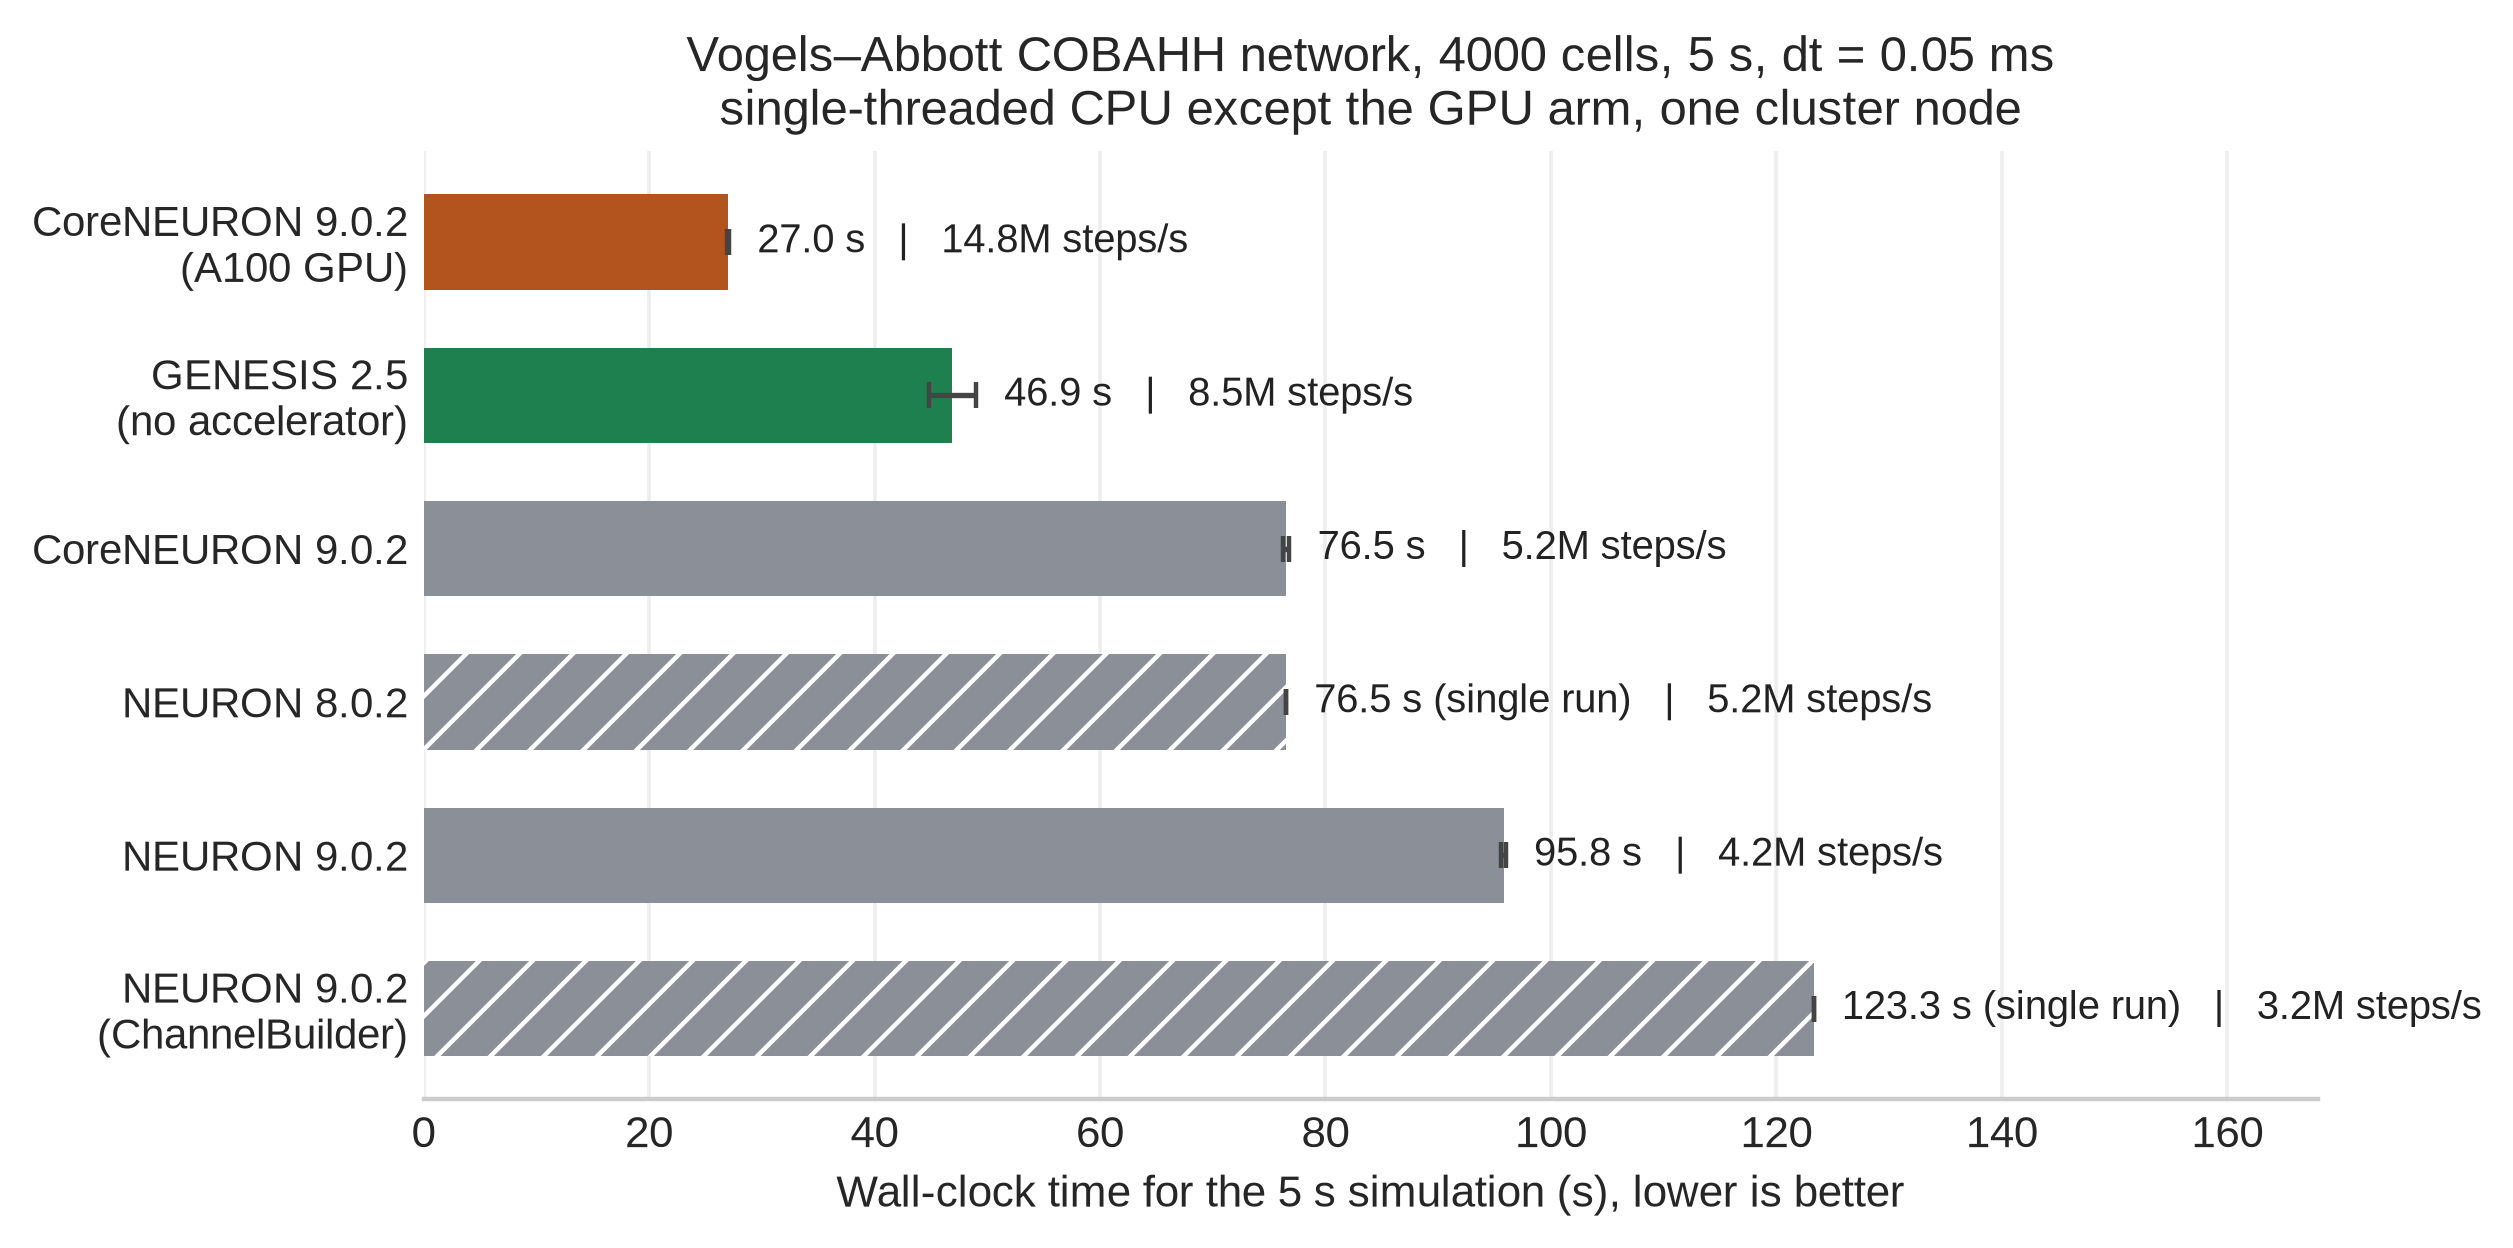
\includegraphics[width=0.92\textwidth]{fig12_coreneuron_comparison.png}
\caption{The measurements of Table~\ref{tab:coreneuron}, drawn. Green is GENESIS, grey the simulators it is compared against; each label names its device, and the dashed guide marks the fastest GENESIS time. Means of 3 replicates, except the ChannelBuilder row.}
\label{fig:coreneuron}
\end{figure}

\textbf{Do the three integrate the same model?} Measured rather than assumed (Fig.~\ref{fig:vmequiv}): NEURON and Arbor agree to $0.02$\,mV at the action-potential peak and to $0.01\%$ on firing rate, while GENESIS peaks $4.6$\,mV lower and fires faster, its Hodgkin--Huxley rates being written about $-70$\,mV where NEURON's use $-65$. Setting the comparison up corrected three errors in our own harness --- Arbor's injection site and its reversal potentials, and a conductance scaled by the soma's area in GENESIS --- none of which moved a wall time by more than $1.3\%$. Timing is unaffected otherwise: with no synapses and no events, switching the injection off moves no arm by $2\%$.

\textbf{GPU against a GPU-native simulator.} In the comparison above the accelerator reaches only parity with its own CPU arm, because a zero-delay spiking network dispatches every step (Section~2.1). To test it where batching does apply we used a model --- $N=10\,000$ neurons, each a chain of 16 compartments, HH channels, current injection, no synapses --- reimplemented in NEURON and in Arbor~\cite{arbor2019}, which was written from scratch for GPU hardware.

Which simulator is faster depends on run length, and the crossover is measurable. Both simulators are linear in $K$ (Table~\ref{tab:mccross}). Fitted over six run lengths, our marginal cost is $33\%$ lower while Arbor starts $0.20$\,s ahead, so the lines cross at $K\approx6400$ (Fig.~\ref{fig:crossover}). Below it Arbor wins on setup; above it, where modelling studies sit, GENESIS~2.5 is faster. The A40 gives the same ordering with a wider margin, crossing at $K\approx1800$: our kernel is fp32 where Arbor computes in double, and that card's double-precision throughput is a fraction of the A100's. A comparison at one run length therefore reports whichever side of the crossing its author chose. The device profile locates the cost: our step phase exceeds kernel time by $0.21$\,s at both run lengths, so it is one-time dispatch setup, not per-step work. This is the cost of the design that keeps existing models working: Arbor generates specialised code per mechanism, while our kernels interpret the \texttt{hsolve} opcode program at run time. On single-threaded CPU the GENESIS solver is $2.02\times$ slower than CoreNEURON here, the opposite of Table~\ref{tab:coreneuron}, because the two benchmarks stress different things: the spiking network is dominated by synaptic event handling over single compartments, this one by the tridiagonal solve, where CoreNEURON's vectorised layout is stronger.

\begin{table}[!h]
\centering
\small
\begin{tabular}{|l|l|r|}
\hline
\textbf{Simulator} & \textbf{Backend} & \textbf{Wall (s)} \\
\hline
\multicolumn{3}{|l|}{\emph{$K=5000$ steps (50\,ms simulated)}} \\
\hline
Arbor 0.10.0 & CPU, 128 threads & 1.09 $\pm$ 0.04 \\
\hline
Arbor 0.10.0 & GPU (A100) & \textbf{1.56 $\pm$ 0.03} \\
\hline
GENESIS 2.5 & GPU (A100) & 1.59 $\pm$ 0.01 \\
\hline
CoreNEURON 9.0.2 & CPU, 1 thread & 60.94 $\pm$ 0.15 \\
\hline
NEURON 9.0.2 & CPU, 1 thread & 82.82 $\pm$ 2.00 \\
\hline
GENESIS 2.5 & CPU, 1 thread & 123.41 $\pm$ 1.75 \\
\hline
\multicolumn{3}{|l|}{\emph{$K=50\,000$ steps (500\,ms simulated)}} \\
\hline
GENESIS 2.5 & \textbf{GPU (A100)} & \textbf{4.56 $\pm$ 0.01} \\
\hline
Arbor 0.10.0 & GPU (A100) & 5.95 $\pm$ 0.02 \\
\hline
\end{tabular}
\caption{The same multi-compartment model in three simulators, on CPU and on GPU, at two run lengths. $N=10\,000$ neurons $\times$ 16 compartments, $dt=0.01$\,ms, UMCS node inf03, mean $\pm$ std over 3 replicates, both arms of every pair timed identically. Thread counts differ and are stated: Arbor uses all cores by default, the others are single-threaded. The CPU arms appear only at $K=5000$, where they were measured; extrapolating them would be an estimate. The GPU rows come from the sweep Fig.~\ref{fig:crossover} fits, so table and figure cannot disagree. The models match in geometry, passive properties, conductances, injection and timestep (Fig.~\ref{fig:vmequiv}); this is a throughput comparison, not a claim of identical trajectories. Harness: \protect\path{cluster_bringup/coreneuron/}.}
\label{tab:mccross}
\end{table}

\begin{figure}[!h]
\centering
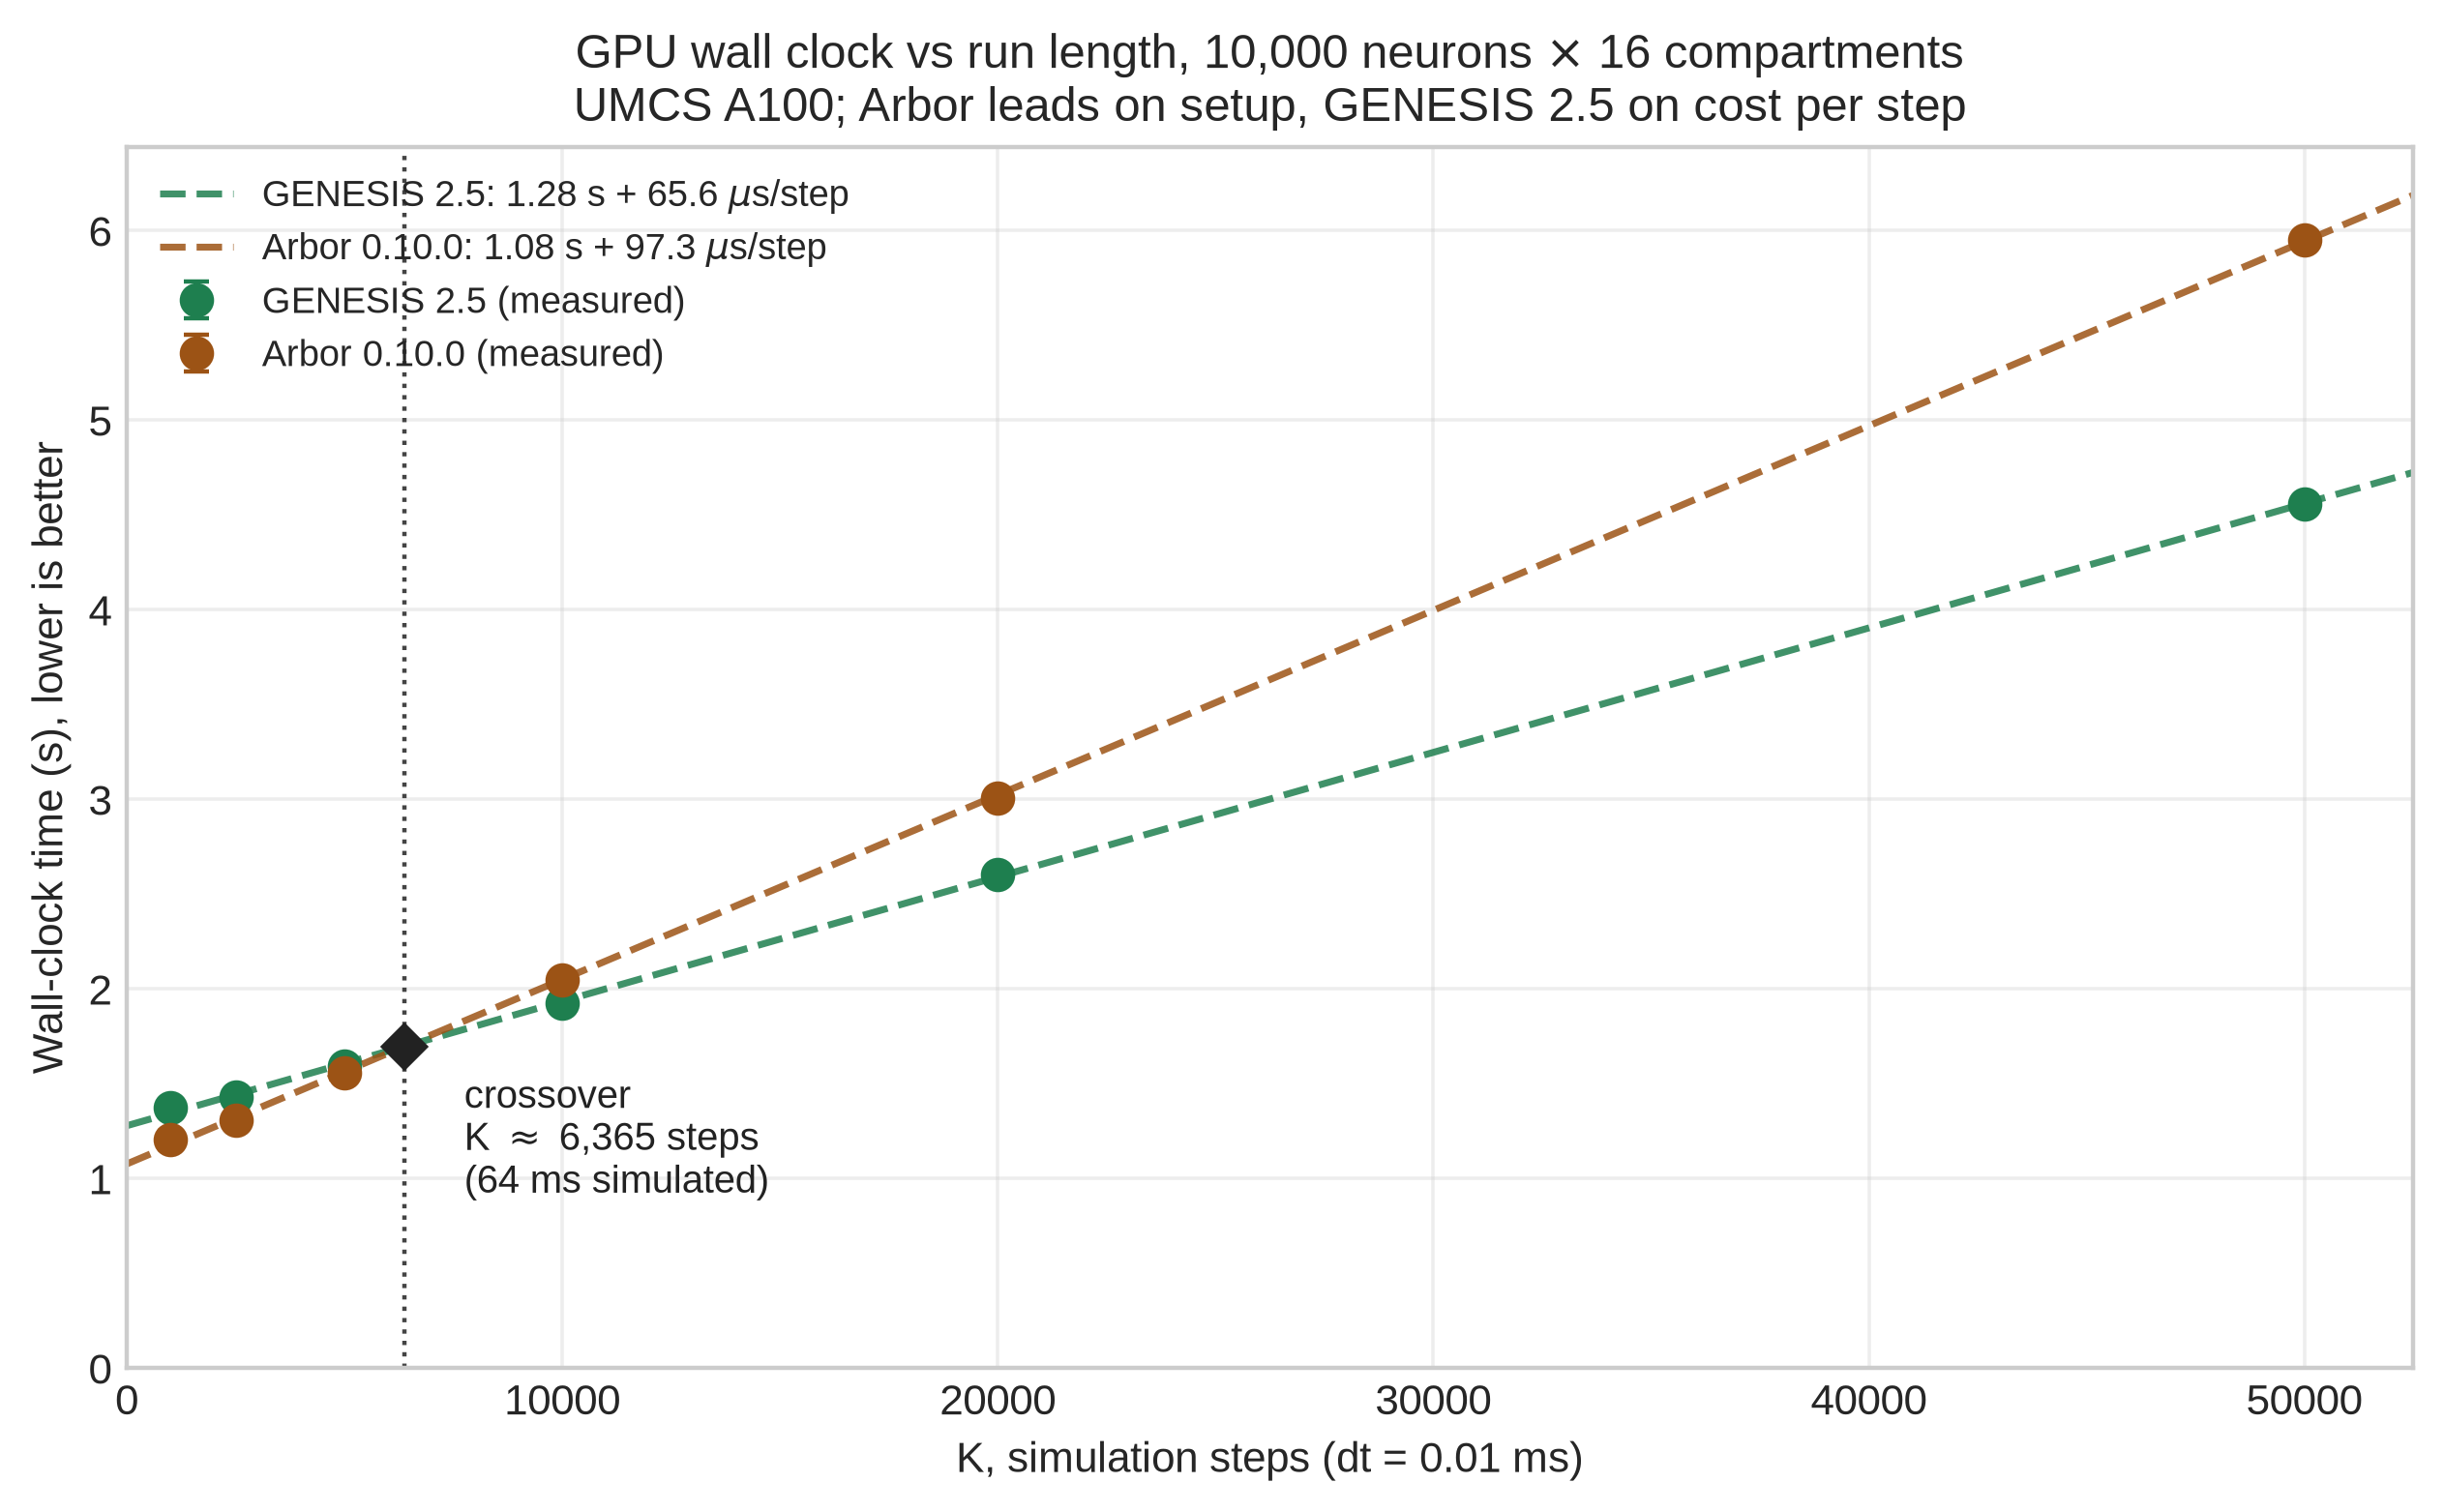
\includegraphics[width=0.85\textwidth]{fig13_crossover.png}
\caption{Wall-clock time against run length for the multi-compartment benchmark, one panel per card, $N=10\,000$ neurons $\times$ 16 compartments, mean $\pm$ std over 3 replicates. The dotted line and diamond mark where the fitted lines cross.}
\label{fig:crossover}
\end{figure}

\begin{figure}[!h]
\centering
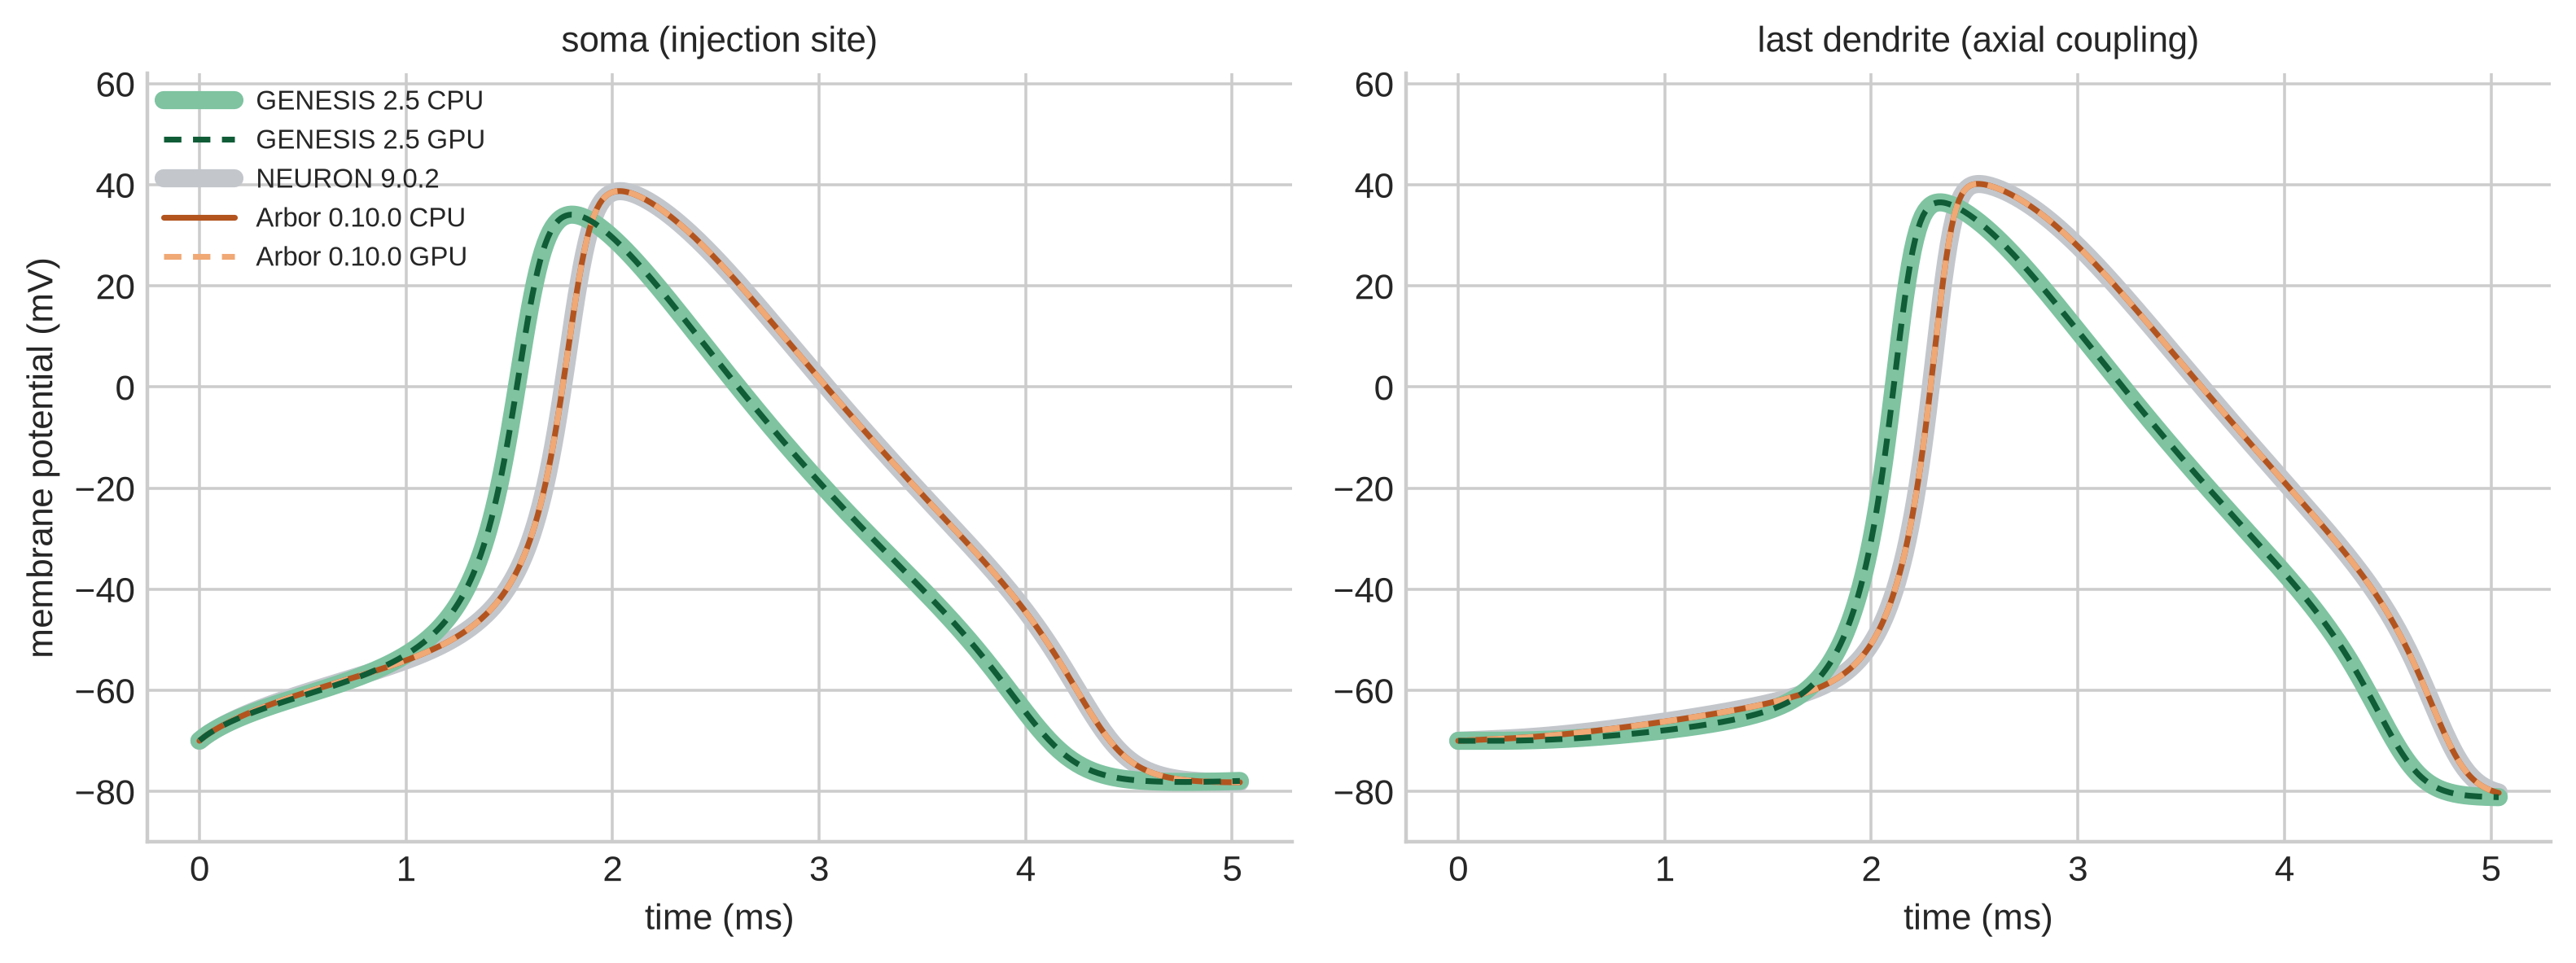
\includegraphics[width=0.98\textwidth]{fig14_vm_equivalence.png}
\caption{One cell's first action potential in three simulators, at the soma and at the far end of the dendrite, which moves only if axial coupling is integrated. Each simulator is drawn twice, one backend wide and pale with the other dashed on top, so a coinciding pair reads as agreement rather than a missing line. Data: \protect\path{cluster_bringup/logs/vmcross/}.}
\label{fig:vmequiv}
\end{figure}

A reproduction pack is included: \path{sh reproduce/run_all.sh} re-measures the claims here on the reader's own hardware, regenerates the figures from those measurements, and prints each published value beside theirs. Two rows need hardware or a toolchain it cannot assume --- CoreNEURON on a GPU, and the A40 arm --- and are documented instead. Raw data and full steps: \path{paper/docs/REPLICATION.md}.

\item Impact

GENESIS/PGENESIS users with channel-kinetics-heavy models now have a path to GPU acceleration (Section~3) without migrating models, SLI scripts, or MPI workflows --- the barrier an architecturally different successor such as MOOSE would impose. The accelerator's scope is deliberate: both kernels interpret the \texttt{hsolve} opcode program directly and implement the five opcodes a current-driven \texttt{tabchannel} model produces, so compartments needing anything else (synaptic channels, a \texttt{spike} element, GHK, concentration pools) are detected at \texttt{SETUP} and computed on the CPU. That boundary defines what this release accelerates, and a published network model is what established where it lies (Section~1).

The correctness and construction fixes reach further than the accelerator does. The three Hines-solver defects silently suppressed \texttt{inject}-driven voltage transients for every neuron but the first in any multi-neuron \texttt{hsolve}, and the five linear-scan patterns behind $O(n^2)$ construction (Section~3) blocked population-scale models outright. Both predate this release and are fixed for every GENESIS/PGENESIS user, whether or not an accelerator is available.


\item Conclusions

GENESIS 2.5 adds opt-in OpenCL and CUDA acceleration to GENESIS 2.4/PGENESIS 2.4 for Hodgkin--Huxley \texttt{tabchannel} models, without changes to model files, SLI scripts, or MPI workflows (Section~3 reports speedup and fidelity on cluster-class hardware). Beyond the single-compartment multiloop kernel, \hte{} extends acceleration to axially-coupled multi-compartment trees at population scale; the single-detailed-cell regime is not helped by this design, which we measure and report.

The release also carries seven correctness fixes to code already in users' hands. Three are Hines-solver defects that silently suppressed \texttt{inject}-driven voltage transients in any multi-neuron \texttt{hsolve}, and benefit any GENESIS/PGENESIS user, accelerator or not; four are in the accelerator as first released (Section~1). Separately, five pre-existing linear-scan patterns compounding into $O(n^2)$ model-construction time are fixed, restoring linear scaling and making population-scale models buildable at all.

Measured against other simulators on a published network model, GENESIS~2.5 is $2.30\times$ faster than CoreNEURON and $2.88\times$ faster than NEURON~9.0.2 for single-threaded CPU execution of the Vogels--Abbott COBAHH benchmark, after verifying that the two implementations are equivalent (Section~3). That benchmark is a spiking network, which this release accelerates for the first time though only to parity with its own CPU arm, so CoreNEURON on an A100 still runs it $1.23\times$ faster. On multi-compartment populations, where the accelerator does apply, GENESIS~2.5 overtakes the GPU-native Arbor beyond 64\,ms of simulated time on an A100 and 18\,ms on an A40.

\textbf{Future work.} Three limits measured here say what to do next, in the order we think they matter to users.

\emph{Parallelism inside the tree.} The kernel gives each tree a thread, so it speeds up populations and does nothing for a single detailed morphology: there only one thread runs, and the GPU is some $20\times$ slower than the CPU. Much of the modelling literature works on exactly that cell, and reaching it needs cyclic reduction or a similar scheme within each tree. This is where the design is furthest from finished.

\emph{Cutting the dispatch.} Lifting the one-spike-generator limit is worth $1.41\times$ on the CPU by itself, and the device then reproduces the network's spike count to $1.1\%$. It does not make it faster. A zero-delay network exchanges spikes every step, so nothing can be batched and each step pays a dispatch, which costs more than the kernel saves: the GPU arm is $1.04\times$ slower than its own CPU. A bigger model does not rescue it --- at 12\,500 cells the two arms are level --- because the accelerable fraction sits near $59\%$ whatever the size, holding the ceiling at $2.4\times$ that dispatch then spends. The work to do is cutting dispatch, not building larger networks.

\emph{Precision over long runs.} fp32 is what lets the kernels run on integrated GPUs with no double-precision hardware, and it costs $\sim$10$^{-7}$\,V against the fp64 CPU over the runs measured here. Whether it stays that small over the far longer runs plasticity studies need is untested.

CoreNEURON's multi-rank MPI configuration is still unmeasured and would place GENESIS~2.5 more completely. Packaging into a container-based deployment pipeline~\cite{chlasta2023pipeline} is in progress.

\end{enumerate}

\section*{CRediT authorship contribution statement}

\textbf{Karol Chlasta}: Conceptualization, Data curation, Formal analysis,
Investigation, Methodology, Project administration, Resources, Software,
Validation, Visualization, Writing -- original draft, Writing -- review and
editing.
\textbf{Grzegorz Marcin W\'ojcik}: Resources, Supervision,
Writing -- review and editing.

\section*{Declaration of competing interest}

The authors declare that they have no known competing financial interests or
personal relationships that could have appeared to influence the work reported
in this paper.

\section*{Declaration of generative AI and AI-assisted technologies in the manuscript preparation process}

During the preparation of this work the authors used Anthropic's Claude to draft and edit the manuscript and to assist with the software and its benchmarking. After using this tool, the authors reviewed and edited the content as needed and take full responsibility for the content of the published article.

\section*{Funding}

This research did not receive any specific grant from funding agencies in the
public, commercial, or not-for-profit sectors.

\section*{Acknowledgements}

The authors thank the Maria Curie-Sk\l{}odowska University (UMCS) in Lublin and
the LubMAN UMCS computing centre for access to the ``Lunar'' cluster (NVIDIA A100
and A40 GPU nodes) at the UMCS Institute of Mathematics, commissioned in
2015~\cite{umcs_lunar2015} and since upgraded with the GPU nodes used in this
work, and Karol S.~Karpowicz and Prof.~Przemys\l{}aw Stpiczy\'nski
for provisioning and support of the compute environment on which the CUDA backend
was built and validated. The authors also thank WarsawIQ for the AMD Radeon~890M
integrated GPU on which the OpenCL backend was developed.

%% The Appendices part is started with the command \appendix;
%% appendix sections are then done as normal sections
%% \appendix

%% \section{}
%% \label{}

%% References:
%% If you have bibdatabase file and want bibtex to generate the
%% bibitems, please use
%%
%% \bibliographystyle{elsarticle-num} 
%% \bibliography{<your bibdatabase>}

%% else use the following coding to input the bibitems directly in the
%% TeX file.

\begin{thebibliography}{9}

\bibitem{bower1998}
Bower~JM, Beeman~D.
\textit{The Book of GENESIS: Exploring Realistic Neural Models with the GEneral NEural SImulation System}.
Springer, 1998.

\bibitem{g3_dev_plans}
GENESIS 3 Development Plans.
\url{http://www.genesis-sim.org/GENESIS/G3/G3-dev-plans.html}

\bibitem{cornelis2011}
Cornelis~H, Coop~AD, Rodriguez~AL, Beeman~D, Bower~JM.
GENESIS 3.0 functionality enhanced by interface to multiple types of database.
\textit{BMC Neuroscience} 2011, 12(Suppl 1):P15.

\bibitem{cornelis2008cbi}
Cornelis~H, Edwards~M, Coop~AD, Bower~JM.
The CBI architecture for computational simulation of realistic neurons and circuits in the GENESIS 3 software federation.
\textit{BMC Neuroscience} 2008, 9(Suppl 1):P88.

\bibitem{cornelis2007dendrite}
Cornelis~H, Lu~H, Esquivel~A, Bower~JM.
Modeling a single dendritic compartment using Neurospaces and GENESIS-3.
\textit{BMC Neuroscience} 2007, 8(Suppl 2):P3.

\bibitem{cornelis2013interop}
Cornelis~H, Bampasakis~D, Steuber~V, Bower~JM.
Interoperability in the GENESIS 3.0 Software Federation: the NEURON Simulator as an Example.
\textit{BMC Neuroscience} 2013, 14(Suppl 1):P33.

\bibitem{arbor2019}
Akar~NA, Cumming~B, Karakasis~V, K\"usters~A, Klijn~W, Peyser~A, Yates~S.
Arbor -- A Morphologically-Detailed Neural Network Simulation Library for Contemporary High-Performance Computing Architectures.
In: \textit{27th Euromicro International Conference on Parallel, Distributed and Network-Based Processing (PDP)}, 2019, pp.~274--282. doi:10.1109/EMPDP.2019.8671560.

\bibitem{kumbhar2019coreneuron}
Kumbhar~P, Hines~M, Fouriaux~J, Ovcharenko~A, King~J, Delalondre~F, Sch\"urmann~F.
CoreNEURON: An Optimized Compute Engine for the NEURON Simulator.
\textit{Frontiers in Neuroinformatics} 2019, 13:63. doi:10.3389/fninf.2019.00063.

\bibitem{markram2015reconstruction}
Markram~H, Muller~E, Ramaswamy~S, et al.
Reconstruction and Simulation of Neocortical Microcircuitry.
\textit{Cell} 2015, 163(2):456--492. doi:10.1016/j.cell.2015.09.029.

\bibitem{hines1984efficient}
Hines~M.
Efficient computation of branched nerve equations.
\textit{International Journal of Bio-Medical Computing} 1984, 15(1):69--76. doi:10.1016/0020-7101(84)90008-4.

\bibitem{hines1997neuron}
Hines~ML, Carnevale~NT.
The NEURON Simulation Environment.
\textit{Neural Computation} 1997, 9(6):1179--1209. doi:10.1162/neco.1997.9.6.1179.

\bibitem{gewaltig2007nest}
Gewaltig~M-O, Diesmann~M.
NEST (NEural Simulation Tool).
\textit{Scholarpedia} 2007, 2(4):1430. doi:10.4249/scholarpedia.1430.

\bibitem{stimberg2019brian}
Stimberg~M, Brette~R, Goodman~DFM.
Brian~2, an intuitive and efficient neural simulator.
\textit{eLife} 2019, 8:e47314. doi:10.7554/eLife.47314.

\bibitem{yavuz2016genn}
Yavuz~E, Turner~J, Nowotny~T.
GeNN: a code generation framework for accelerated brain simulations.
\textit{Scientific Reports} 2016, 6:18854. doi:10.1038/srep18854.

\bibitem{vogels2005signal}
Vogels~TP, Abbott~LF.
Signal Propagation and Logic Gating in Networks of Integrate-and-Fire Neurons.
\textit{Journal of Neuroscience} 2005, 25(46):10786--10795. doi:10.1523/JNEUROSCI.3508-05.2005.

\bibitem{brette2007simulation}
Brette~R, Rudolph~M, Carnevale~T, Hines~M, Beeman~D, Bower~JM, et al.
Simulation of networks of spiking neurons: A review of tools and strategies.
\textit{Journal of Computational Neuroscience} 2007, 23(3):349--398. doi:10.1007/s10827-007-0038-6.

\bibitem{chlasta2023pipeline}
Chlasta~K, Sochaczewski~P, W\'ojcik~GM, Krejtz~I.
Neural simulation pipeline: Enabling container-based simulations on-premise and in public clouds.
\textit{Frontiers in Neuroinformatics} 2023, 17:1122470. doi:10.3389/fninf.2023.1122470.

\bibitem{umcs_lunar2015}
Maria Curie-Sk{\l}odowska University (UMCS), Instytut Matematyki.
Superkomputer LUNAR uruchomiony w Instytucie Matematyki UMCS.
\url{https://www.umcs.pl/pl/aktualnosci,57,superkomputer-lunar-uruchomiony-w-instytucie-matematyki-umcs,27879.chtm}, 2015.

\end{thebibliography}


\section*{Current executable software version}

Not applicable; this release is distributed as source code only (see Current code version above).


\end{document}
\endinput
%%
%% End of file `SoftwareX_article_template.tex'.
